\subsection{Combination of Genres}
\label{ssec:genres_combo}

In the previous section, we looked at how the $\theta_{pos}$ score changes when data from one genre is compared against another. In this subsection, we study how the different genres in combination with each other affect the $\theta_{pos}$ scores.

We denoted the set of genres in treebank $X$ as $G_{X}$. Given two treebanks $A$ and $B$ with at least one different genre, the different genres in the two treebanks $G_{A}$ and $G_{B}$ can be either of the three cases as shown in Figure \ref{fig:GA and GB interactions}.


\begin{figure}[H]
    \begin{subfigure}{.45\textwidth}
        \centering
        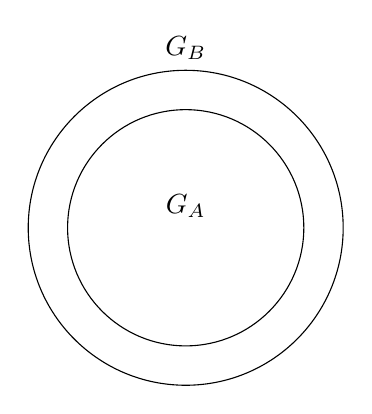
\begin{tikzpicture}[]
            \def\firstcircle{(-1.2,0) coordinate (a) circle (2cm)}
            \def\secondcircle{(-1.2,0) coordinate (b)  circle (1.5cm)}
                \begin{scope}
            \clip \secondcircle;
                \end{scope}
            \draw \firstcircle node[text=black,above] {$G_{A}$};
            \draw \secondcircle;
            \node (c) [above] at (current bounding box.north -| b) {$G_{B}$};
            % \node at (c -| b) {$G_{B}$};
        \end{tikzpicture}
        \caption{Case 1: $G_{A} \subseteq G_{B}$}
        \label{fig:case 1 ga gb}
    \end{subfigure}
    \begin{subfigure}{.5\textwidth}
        \centering
        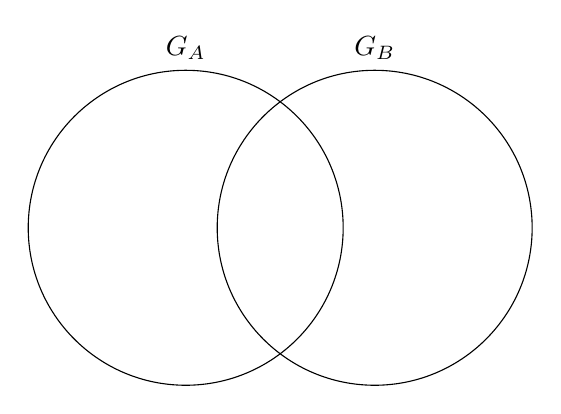
\begin{tikzpicture}[]
            \def\firstcircle{(-1.2,0) coordinate (a) circle (2cm)}
            \def\secondcircle{(1.2,0) coordinate (b)  circle (2cm)}
                \begin{scope}
            \clip \secondcircle;
                \end{scope}
            \draw \firstcircle;
            \draw \secondcircle;
            \node (c) [above] at (current bounding box.north -| a) {$G_{A}$};
            \node at (c -| b) {$G_{B}$};
        \end{tikzpicture}
        \caption{Case 2: $G_{A} \not \subseteq G_{B}$; $G_{A} \cap G_{B} \neq \phi$}
        \label{fig:case 2 ga gb}
    \end{subfigure}
    \newline
    \begin{subfigure}{\textwidth}
        \centering
        \begin{tikzpicture}[]
            \def\firstcircle{(-3,0) coordinate (a) circle (2cm)}
            \def\secondcircle{(3,0) coordinate (b)  circle (2cm)}
                \begin{scope}
            \clip \secondcircle;
                \end{scope}
            \draw \firstcircle;
            \draw \secondcircle;
            \node (c) [above] at (current bounding box.north -| a) {$G_{A}$};
            \node at (c -| b) {$G_{B}$};
        \end{tikzpicture}
        \caption{Case 3: $G_{A} \not \subseteq G_{B}$; $G_{A} \cap G_{B} = \phi$}
        \label{fig:case 3 ga gb}
    \end{subfigure}
    \caption{Interaction of Genres in Treebanks $A$ and $B$, such that $\vert G_{A} \vert \leq \vert G_{B} \vert$}
    \label{fig:GA and GB interactions}
\end{figure}

To see how the $\theta_{pos}$ scores are affected in either of the cases, we perform the following experiment on UDv2.5 \texttt{pl}-LFG data.

\begin{enumerate}
    \item Downsample the number of sentences in \textit{fiction} and \textit{news} genres to 2000 sentences each. Using 2-fold cross-validation, split the downsampled into 2 halves. We refer to one half as \textit{base} set for the genre, and the other as the \textit{test} set for the genre, each containing 1000 sentences.
    \item Downsample the number of sentences in \textit{spoken} genre to 1000 sentences.
    \item Concatenate the downsampled \textit{spoken} data and the \textit{test} set from the other genres. Refer to this dataset as \textit{all\_genres}.
        \begin{equation*}
            \textit{all\_genres} = \textit{spoken} + \textit{fiction\_test} + \textit{news\_test}
        \end{equation*}
    \item Combine the \textit{test} sets to result in \textit{news\_fiction\_test} set.
        \begin{equation*}
            \textit{news\_fiction\_test} = \textit{news\_test} + \textit{fiction\_test}
        \end{equation*}
    \item Combine the \textit{base} sets to result in \textit{news\_fiction\_base} set.
        \begin{equation*}
            \textit{news\_fiction\_base} = \textit{news\_base} + \textit{fiction\_base}
        \end{equation*}
    \item Combine the downsampled \textit{spoken} data with either \textit{test} set to result in \textit{spoken\_genre\_test} data, where \textit{genre} is a placeholder for either of \textit{fiction} or \textit{news}.
        \begin{align*}
            \textit{spoken\_news\_test} & = \textit{spoken} + \textit{news\_test}\\
            \textit{spoken\_fiction\_test} &= \textit{spoken} + \textit{fiction\_test}
        \end{align*}
    \item For Case 1, we study the change in $\theta_{pos}$ score when the data as mentioned in Table \ref{tab:case1_genre} are compared against each other.
        \begin{table}[H]
            \centering
            \begin{tabular}{|c|c|}
                \hline
                \textbf{$G_{A}$} & \textbf{$G_{B}$} \\
                \hline
                $G_{news\_base} = \{news\}$ & $G_{news\_fiction\_test} = \{news, fiction\}$\\
                $G_{news\_base} = \{news\}$ & $G_{spoken\_news\_test} = \{spoken, news\}$\\
                $G_{news\_base} = \{news\}$ & $G_{all\_genres} = \{news, fiction, spoken\}$\\
                \hline
                $G_{fiction\_base} = \{fiction\}$ & $G_{news\_fiction\_test} = \{news, fiction\}$\\
                $G_{fiction\_base} = \{fiction\}$ & $G_{spoken\_fiction\_test} = \{spoken, fiction\}$\\
                $G_{fiction\_base} = \{fiction\}$ & $G_{all\_genres} = \{news, fiction, spoken\}$\\
                \hline
                $G_{news\_fiction\_base} = \{news, fiction\}$ & $G_{all\_genres} = \{news, fiction, spoken\}$\\
                \hline
            \end{tabular}
            \caption{Datasets Compared when $G_{A} \subset G_{B}$ and $\vert G_{A} \vert < \vert G_{B} \vert$}
            \label{tab:case1_genre}
        \end{table}
    \item For Case 2, we study the change in $\theta_{pos}$ score when the data as mentioned in Table \ref{tab:case2_genre} are compared against each other.
        \begin{table}[H]
            \centering
            \begin{tabular}{|c|c|}
                \hline
                \textbf{$G_{A}$} & \textbf{$G_{B}$} \\
                \hline
                $G_{news\_fiction\_base} = \{news, fiction\}$ & $G_{spoken\_news\_test} = \{spoken, news\}$\\
                $G_{news\_fiction\_base} = \{news, fiction\}$ & $G_{spoken\_fiction\_test} = \{spoken, fiction\}$\\
                \hline
            \end{tabular}
            \caption{Datasets Compared when $G_{A} \not \subseteq G_{B}$; $G_{A} \cap G_{B} \neq \phi$ and $\vert G_{A} \vert \leq \vert G_{B} \vert$}
            \label{tab:case2_genre}
        \end{table}
    \item For Case 3, we study the combinations as listed in Table \ref{tab:case3_genre}.
        \begin{table}[H]
            \centering
            \begin{tabular}{|c|c|}
                \hline
                \textbf{$G_{A}$} & \textbf{$G_{B}$} \\
                \hline
                $G_{news\_base} = \{news\}$ & $G_{spoken\_fiction\_test} = \{spoken, fiction\}$\\
                $G_{fiction\_base} = \{fiction\}$ & $G_{spoken\_news\_test} = \{spoken, news\}$\\
                $G_{spoken} = \{spoken\}$ & $G_{news\_fiction\_test} = \{news, fiction\}$\\
                \hline
            \end{tabular}
            \caption{Datasets Compared when $G_{A} \not \subseteq G_{B}$; $G_{A} \cap G_{B} = \phi$ and $\vert G_{A} \vert \leq \vert G_{B} \vert$}
            \label{tab:case3_genre}
        \end{table}
    \item We also calculate $\theta_{pos}$ scores for each \textit{base} and \textit{test} sets with each other, and with \textit{spoken} data, to better know how the scores are being impacted.
    \item We repeat all the above steps 100 times, each with a different seed value to result in differently downsampled data. We present the calculated scores averaged over 100 runs for different cases in Tables \ref{tab:case1_genre-results} - \ref{tab:case3_genre-results}. In the tables, the `Average' column contains the average of means from the preceding columns.
\end{enumerate}

\begin{table}[H]
    \centering
    \begin{tabular}{|c|c|c|c|c|}
        \hline
         & \textit{news\_test} & \textit{fiction\_test} & Average & \textit{news\_fiction\_test}\\
        \hline
        \textit{news\_base} & 0.257 ± 0.01 & 0.646 ± 0.034 & 0.452 & 0.304 ± 0.016 \\
        \textit{fiction\_base} & 0.64 ± 0.034 & 0.278 ± 0.013 & 0.46 & 0.348 ± 0.019 \\
        \hline
    \end{tabular}%
    \vspace{5mm}
    \begin{tabular}{|c|c|c|c|c|}
        \hline
         & \textit{news\_test} & \textit{spoken} & Average & \textit{spoken\_news\_test}\\
        \hline
        \textit{news\_base} & 0.257 ± 0.01 & 1.503 ± 0.049 & 0.88 & 0.489 ± 0.022\\
        \hline
    \end{tabular}%
    \vspace{5mm}
    \begin{tabular}{|c|c|c|c|c|}
        \hline
         & \textit{fiction\_test} & \textit{spoken} & Average & \textit{spoken\_fiction\_test}\\
        \hline
        \textit{fiction\_base} & 0.278 ± 0.013 & 0.99 ± 0.036 & 0.63 & 0.41 ± 0.018\\
        \hline
    \end{tabular}%
    \vspace{5mm}
    \scalebox{0.8}{\begin{tabular}{|c|c|c|c|c|c|}
        \hline
         & \textit{news\_test} & \textit{fiction\_test} & \textit{spoken} & Average & \textit{all\_genres}\\
        \hline
        \textit{news\_base} & 0.257 ± 0.01 & 0.646 ± 0.034 & 1.503 ± 0.049 & 0.802 & 0.463 ± 0.022\\
        \textit{fiction\_base} & 0.64 ± 0.034 & 0.278 ± 0.013 & 0.99 ± 0.036 & 0.64 & 0.351 ± 0.014\\
        \textit{news\_fiction\_base} & 0.3 ± 0.015 & 0.351 ± 0.021 & 1.144 ± 0.035 & 0.6 & 0.247 ± 0.011\\
        \hline
    \end{tabular}}
    \caption{$\theta_{pos}$ ($\pm$ sd) Scores Averaged over 100 Runs, Reported for Case When $G_{A} \subset G_{B}$ and $\vert G_{A} \vert < \vert G_{B} \vert$}
    \label{tab:case1_genre-results}
\end{table}

\begin{table}[H]
    \centering
    \scalebox{0.9}{\begin{tabular}{|c|c|c|c|c|}
        \hline
         & \textit{spoken} & \textit{news\_test} & Average & \textit{spoken\_news\_test}\\
        \hline
        \textit{news\_base} & 1.503 ± 0.049 & 0.257 ± 0.01 & 0.88 & 0.489 ± 0.022\\
        \textit{fiction\_base} & 0.99 ± 0.036 & 0.64 ± 0.034 & 0.81 & 0.499 ± 0.02\\
        \textit{news\_fiction\_base} & 1.144 ± 0.035 & 0.3 ± 0.015 & 0.7 & 0.498 ± 0.023\\
        \hline
    \end{tabular}}%
    \vspace{5mm}
    \scalebox{0.9}{\begin{tabular}{|c|c|c|c|c|}
        \hline
         & \textit{spoken} & \textit{fiction\_test} & Average & \textit{spoken\_fiction\_test}\\
        \hline
        \textit{news\_base} & 1.503 ± 0.049 & 0.646 ± 0.034 & 1.075 & 0.854 ± 0.036\\
        \textit{fiction\_base} & 0.99 ± 0.036 & 0.278 ± 0.013 & 0.63 & 0.41 ± 0.018\\
        \textit{news\_fiction\_base} & 1.144 ± 0.035 & 0.351 ± 0.021 & 0.747 & 0.498 ± 0.023\\
        \hline
    \end{tabular}}
    \caption{$\theta_{pos}$ ($\pm$ sd) Scores Averaged over 100 Runs, Reported for Case When $G_{A} \not \subseteq G_{B}$; $G_{A} \cap G_{B} \neq \phi$ and $\vert G_{A} \vert \leq \vert G_{B} \vert$}
    \label{tab:case2_genre-results}
\end{table}

\begin{table}[H]
    \centering
    \begin{tabular}{|c|c|c|c|c|}
        \hline
         & \textit{spoken} & \textit{fiction\_test} & Average & \textit{spoken\_fiction\_test}\\
        \hline
        \textit{news\_base} & 1.503 ± 0.049 & 0.646 ± 0.034 & 1.075 & 0.854 ± 0.036\\
        \hline
    \end{tabular}%
    \vspace{5mm}
    \begin{tabular}{|c|c|c|c|c|}
        \hline
         & \textit{spoken} & \textit{news\_test} & Average & \textit{spoken\_news\_test}\\
        \hline
        \textit{fiction\_base} & 0.99 ± 0.036 & 0.64 ± 0.034 & 0.81 & 0.499 ± 0.02\\
        \hline
    \end{tabular}%
    \vspace{5mm}
    \begin{tabular}{|c|c|c|c|c|}
        \hline
         & \textit{news\_test} & \textit{fiction\_test} & Average & \textit{news\_fiction\_test}\\
        \hline
        \textit{spoken} & 1.493 ± 0.048 & 0.987 ± 0.034 & 1.24 & 1.138 ± 0.03\\
        \hline
    \end{tabular}
    \caption{$\theta_{pos}$ ($\pm$ sd) Scores Averaged over 100 Runs, Reported for Case When $G_{A} \not \subseteq G_{B}$; $G_{A} \cap G_{B} = \phi$ and $\vert G_{A} \vert \leq \vert G_{B} \vert$}
    \label{tab:case3_genre-results}
\end{table}

From the tables, it can be observed that the decomposition of a treebank into its constituent genres forms the first basis for the combination of the different genres. Once the individual genres have been identified and checked for the inter-generic $\theta_{pos}$ scores, the overall metric score is less than the average of the metric scores calculated for individual pair of genres in the treebank(s). Upon a closer inspection, it was discovered that when there are multiple genres present in the treebank, the $\theta_{pos}$ metric score is dominated by the POS trigrams that are typical of the language, and the genre-specific POS trigrams become more and more obscure.

Assuming treebanks $A$ and $B$ can be split into their constituent genres such that $G_{A} = \{A_{1}, A_{2}, ... , A_{i}\}$ and $G_{B} = \{B_{1}, B_{2}, ... , B_{j}\}$, the overall limit on the $\theta_{pos}(A, B)$ score can be specified as in Equation \ref{eqn:theta_pos_combo_limit}.

\begin{equation}
    \boxed{\theta_{pos}(A, B) \leq \Theta_{pos}(A, B) = Average(\theta_{pos}(A_{x}, B_{y}))} \hspace{5mm} \forall [A_{x} \in G_{A}; B_{y} \in G_{B}]
\label{eqn:theta_pos_combo_limit}
\end{equation}

\subsection{Adulterant Genres in Dataset}
\label{sec:adulterant}

In our analysis so far, we have restricted ourselves to instances when the data in the different genres could be reliably compared as per Equation \ref{eqn:size_constraint} reproduced below:

\begin{equation}
\boxed{size(A) \geq 400 \And Avg(A) \geq Avg(B) \implies size(B) \cdot \frac{Avg(B)}{Avg(A)} \geq 400} \tag{\ref{eqn:size_constraint}}
\end{equation}

 where

\begin{enumerate}
    \item $Avg(X) = \frac{Total Syntactic Words(X)}{size(X)}$ is the average sentence length in dataset $X$
    \item $size(X)$ refers to the number of sentences in dataset $X$
\end{enumerate}


We define a genre as an adulterant genre in the dataset if the number of instances in the genre don't satisfy Equation \ref{eqn:size_constraint}. In this subsection, we take a look at how the presence of adulterant genres affect the $\theta_{pos}$ scores.

From Table \ref{tab:inter_genre-pl}, the maximal $\theta_{pos}$ score of $1.53$ was computed between \textit{news} and \textit{spoken} genres in data from \texttt{pl}-LFG treebank. We calculate the effect of the adulterant genres in the following manner:

\begin{enumerate}
    \item Downsample data from \textit{fiction}, \textit{news} and \textit{spoken} genres in \texttt{pl}-LFG treebank to 500, 500 and 600 sentences respectively.
    \item Concatenate data from each of \textit{academic}, \textit{blog} and \textit{legal} genres with the downsampled \textit{fiction} dataset to result in \textit{fiction-academic}, \textit{fiction-blog}, and \textit{fiction-legal} datasets.
    \item Repeat Step2 above after replacing downsampled \textit{fiction} dataset with the downsampled \textit{news} dataset to result in \textit{news-academic}, \textit{news-blog}, and \textit{news-legal} datasets.
    \item Concatenate the downsampled datasets from \textit{fiction} and \textit{news} genre to result in \textit{fiction\_news} dataset.
    \item Concatenate data from each of \textit{academic}, \textit{blog}, \textit{legal} genres with the  \textit{fiction\_news} dataset to result in \textit{fiction\_news-academic}, \textit{fiction\_news-blog} and \textit{fiction\_news-legal} datasets.
    \item Concatenate \textit{academic}, \textit{blog} and \textit{legal} datasets to result in a \textit{others} dataset.
    \item Concatenate downsampled \textit{fiction} dataset with the \textit{others} dataset to result in \textit{fiction-others} dataset.
    \item Repeat Step7 above after replacing downsampled \textit{fiction} dataset with downsampled \textit{news} dataset to result in \textit{news-others} dataset.
    \item Concatenate downsampled \textit{fiction} and \textit{news} datasets with the \textit{others} dataset to result in a \textit{all-genres} dataset.
    \item Calculate $\theta_{pos}$ score of downsampled \textit{spoken} dataset with each of the created datasets.
\end{enumerate}

\begin{table}[H]
    \centering
    \begin{tabular}{|l|c|}
        \hline
         & \textit{spoken} \\
         \hline
        \textit{fiction} & 1.059 ± 0.047 \\
        \textit{fiction-academic} & 1.072 ± 0.046 \\
        \textit{fiction-blog} & 1.09 ± 0.044 \\
        \textit{fiction-legal} & 1.065 ± 0.047 \\
        \textit{fiction-others} & 2.413 ± 0.384 \\
        \hline
    \end{tabular}%
    \hspace{1mm}
    \begin{tabular}{|l|c|}
        \hline
         & \textit{spoken} \\
         \hline
        \textit{news} & 1.53 ± 0.071 \\
        \textit{news-academic} & 1.552 ± 0.069 \\
        \textit{news-blog} & 1.54 ± 0.065 \\
        \textit{news-legal} & 1.547 ± 0.071 \\
        \textit{news-others} & 2.63 ± 0.334 \\
        \hline
    \end{tabular}%
    \vspace{5mm}
    \begin{tabular}{|l|c|}
        \hline
         & \textit{spoken} \\
         \hline
        \textit{fiction} & 1.059 ± 0.047 \\
        \textit{news} & 1.53 ± 0.071 \\
        \textit{fiction\_news} & 1.196 ± 0.048 \\
        \textit{fiction\_news-academic} & 1.215 ± 0.048 \\
        \textit{fiction\_news-blog} & 1.223 ± 0.046 \\
        \textit{fiction\_news-legal} & 1.206 ± 0.048 \\
        \textit{all-genres} & 2.309 ± 0.358 \\
        \hline
    \end{tabular}
    \caption{$\theta_{pos}$ Scores ($\pm$ sd) Averaged over 100 Different Runs With Adulterant Genres are Present in \texttt{pl}-LFG Data}
    \label{tab:adulterant-scores}
\end{table}

We observe that a lower number of adulterant genres in the data don't affect the $\theta_{pos}$ scores heavily. However, the presence of multiple adulterant genres pushes the $\theta_{pos}$ scores by almost $1.5$ as compared to when there are no adulterants present. Taking into account also the standard deviation score, and the high annotation quality of the treebank, we can add a headroom of $\pm 2$ if adulterant genres are present. 

Assuming treebanks $A$ and $B$ can be split into their constituent genres such that $G_{A} = \{A_{1}, A_{2}, ... , A_{n1}\}$ and $G_{B} = \{B_{1}, B_{2}, ... , B_{n2}\}$. Of these constituent genres, at least $k$ genres in $G_{A} \cup G_{B}$ are adulterant genres, represented by set of adulterant genres $G_{adulterant}$. The overall limit on the $\theta_{pos}(A, B)$ score, as specified in Equation \ref{eqn:theta_pos_combo_limit}, can be updated as in Equation \ref{eqn:theta_pos_combo_limit_final}.

\begin{equation}
    \boxed{\theta_{pos}(A, B) \leq \Theta_{pos}(A, B) = \begin{cases}
    Average(\theta_{pos}(A_{x}, B_{y})) + 2.0 & \text{if } G_{adulterant} \neq \phi\\
    \vspace{2mm}\\
    Average(\theta_{pos}(A_{x}, B_{y})) & \text{if } G_{adulterant} = \phi\\
    \end{cases}}
\label{eqn:theta_pos_combo_limit_final}
\end{equation}
\hfill $\forall [A_{x}, B_{y} \in (G_{A} \cup G_{B}) - G_{adulterant}]$

\section{Framing Overall \texorpdfstring{$\Theta_{pos}$}{Theta\_pos} Limit}
\label{sec:pos-harmony-calculations}

We studied the effects of size and genre variation in treebanks in the previous sections. It was stated earlier that in order for two datasets to be compared, they should satisfy the condition as mentioned in Equation \ref{eqn:size_constraint} (restated below).

\begin{equation}
\boxed{size(A) \geq 400 \And Avg(A) \geq Avg(B) \implies size(B) \cdot \frac{Avg(B)}{Avg(A)} \geq 400} \tag{\ref{eqn:size_constraint}}
\end{equation}

 where

\begin{enumerate}
    \item $Avg(X) = \frac{Total Syntactic Words(X)}{size(X)}$ is the average sentence length in dataset $X$
    \item $size(X)$ refers to the number of sentences in dataset $X$
\end{enumerate}

For given datasets of the same genre such that the datasets satisfy the condition in Equation \ref{eqn:size_constraint} above, the upper limit on the $\theta_{pos}$ metric score for the datasets to be deemed as consistent in their annotation is specified in Equation \ref{eqn:theta_pos_size_limit} (restated below).

\begin{equation}
\boxed{\theta_{pos}(A,B) \leq \Theta_{pos}(A,B) = 0.5}  \tag{\ref{eqn:theta_pos_size_limit}}
\end{equation}

For the different genres that are present in two treebanks, if the number of instances in the genre do not satisfy Equation \ref{eqn:size_constraint}, we call it as an adulterant genre. In case of multiple genres being present in either treebank under consideration, the upper limit on $\theta_{pos}$ scores is determined on basis of whether or not there is an adulterant genre present as per Equation \ref{eqn:theta_pos_combo_limit_final} reproduced below:

\begin{equation}
    \boxed{\theta_{pos}(A, B) \leq \Theta_{pos}(A, B) = \begin{cases}
    Average(\theta_{pos}(A_{x}, B_{y})) + 2.0 & \text{if } G_{adulterant} \neq \phi\\
    \vspace{2mm}\\
    Average(\theta_{pos}(A_{x}, B_{y})) & \text{if } G_{adulterant} = \phi\\
    \end{cases}}
\tag{\ref{eqn:theta_pos_combo_limit_final}}
\end{equation}
\hfill $\forall [A_{x}, B_{y} \in (G_{A} \cup G_{B}) - G_{adulterant}]$

where $\theta_{pos}(A_{x}, B_{y})$ refers to the calculated $\theta_{pos}$ score calculated between genre $x$ present in treebank $A$ and genre $y$ present in treebank $B$. The upper limit on individual $\theta_{pos}$ value between two genres $A_{x}$ and $B_{y}$ for the genres to be declared consistent with each other is given by Equation \ref{eqn:theta_pos_genre_limit} as stated below:

\begin{equation}
    \boxed{\theta_{pos}(A_{x}, B_{y}) \leq \Theta_{pos}(A_{x}, B_{y}) = 2.0}
\tag{\ref{eqn:theta_pos_genre_limit}}
\end{equation}

Regardless of the genre composition of the treebanks under consideration, the treebanks with $\theta_{pos}$ score $\leq 0.5$ are termed as consistent with respect to their POS annotation. Similarly, the treebanks with $\theta_{pos}$ score $\geq 4.0$ are termed as inconsistent with respect to their POS annotation. If both the treebanks under consideration contain a singular genre each (i.e. $\vert G_{A} \vert = \vert G_{B} \vert = 1$), they would be termed as inconsistent in their POS annotation if their $\theta_{pos} \geq 2$. For all other treebanks, a crude estimate on whether the POS annotation of a treebank is consistent with other treebank(s) or not can be made if just the percentage composition of different genres in the treebanks is known, regardless of whether it is possible to split the treebank into the constituent genres. However, for a fine-tuned estimation, it is imperative to be able to split the treebank into its constituent genres. 

For estimating the annotation consistency of a given pair of treebanks, we proceed as follows:
\begin{enumerate}
    \item If the $\theta_{pos}$ score of the pair of the treebanks is less than or equal to 0.5, the treebanks are pronounced as consistent in their POS annotation with respect to each other.
    \item If the $\theta_{pos}$ score of the pair of the treebanks is greater than or equal to 4.0, the treebanks are pronounced as inconsistent in their POS annotation with respect to each other.
    \item If possible, split the treebanks into the constituent genres.
    \item Isolate the adulterant genres, if any, and calculate $\theta_{pos}$ scores taking one genre from the remaining genres in either treebank and average the resultant scores. The $\Theta_{pos}$ value is calculated as per Equation \ref{eqn:theta_pos_combo_limit_final}.
    \item In case the split into constituent genres is not possible but the percentage composition of the constituent genres is known, estimate the upper limit of the pair of genres from either treebank as per Equations \ref{eqn:theta_pos_size_limit} and \ref{eqn:theta_pos_genre_limit}. The $\Theta_{pos}$ limit is the calculated on the average of these estimated values.
    \item In case the percentage composition of different genres is not known either, we cannot estimate the $\Theta_{pos}$ limit.
    \item Based on the calculated $\Theta_{pos}$ limit and the $\theta_{pos}$ value of the pair of treebanks, the treebanks can be pronounced as consistent or inconsistent, as the case may be.
\end{enumerate}

\section{\texorpdfstring{$\theta_{pos}$}{theta\_pos} Scores for UDv2.5, Annotated To Mark Consistent And Inconsistent Treebanks}
\label{sec:theta_pos_annotations}

This section lists the $\theta_{pos}$ scores in UDv2.5 data \citep{UDv2.5}, as listed earlier in Section \ref{sec:pos-harmony-scores}. Instead of just listing the scores, the scores are color coded as per Table \ref{tab:color-codes} below.

\begin{table}[H]
    \centering
    \begin{tabular}{|c|l|}
        \hline
        \textbf{Color} & \textbf{Significance} \\
        \hline
        \cellcolor{red!25}Red & Inconsistent in POS Annotation\\
        \hline
        \cellcolor{green!25}Green & Consistent in POS Annotation\\
        \hline
        \cellcolor{gray!25}Gray & Could Not Be Estimated\\
        \hline
    \end{tabular}
    \caption{Color Codes Used to Mark Consistent or Inconsistent Treebanks based on $\theta_{pos}$ Scores in Table \ref{tab:theta-pos-again}}
    \label{tab:color-codes}
\end{table}

\begin{minipage}{0.485\textwidth}
\begin{table}[H]
    \scalebox{0.90}{\begin{tabular}{|l|l|l|}
    \hline
    \textbf{Treebank1} & \textbf{Treebank2} & \textbf{$\theta_{pos}$} \\
    \hline
    \texttt{ar}-NYUAD & \texttt{ar}-PADT & \cellcolor{red!25}2.497\\
    \hline
    \texttt{es}-AnCora & \texttt{es}-GSD & \cellcolor{green!25}0.352\\
    \hline
    \texttt{et}-EDT & \texttt{et}-EWT & \cellcolor{green!25}0.413\\
    \hline
    \texttt{fi}-FTB & \texttt{fi}-TDT & \cellcolor{red!25}1.195\\
    \hline
    \cellcolor{blue!25}\texttt{gl}-CTG & \texttt{gl}-TreeGal & \cellcolor{blue!25}0.714\\
    \hline
    \texttt{grc}-Perseus & \texttt{grc}-PROIEL & \cellcolor{red!25}4.641\\
    \hline
    \texttt{ja}-BCCWJ & \cellcolor{gray!25}\texttt{ja}-GSD & \cellcolor{gray!25}0.951\\
    \hline
    \cellcolor{gray!25}\texttt{ko}-GSD & \texttt{ko}-Kaist & \cellcolor{gray!25}2.56\\
    \hline
    \texttt{nl}-Alpino & \texttt{nl}-LassySmall & \cellcolor{green!25}0.664\\
    \hline
    \texttt{pl}-LFG & \cellcolor{blue!25}\texttt{pl}-PDB & \cellcolor{blue!25}0.623\\
    \hline
    \texttt{pt}-Bosque & \cellcolor{gray!25}\texttt{pt}-GSD & \cellcolor{gray!25}0.678\\
    \hline
    \texttt{ro}-Nonstandard & \texttt{ro}-RRT & \cellcolor{green!25}1.233\\
    \hline
    \texttt{sl}-SSJ$^{+}$ & \texttt{sl}-SST & \cellcolor{green!25}2.405\\
    \hline
    \texttt{sv}-LinES & \texttt{sv}-Talbanken & \cellcolor{green!25}0.443\\
    \hline
    \texttt{tr}-GB & \cellcolor{blue!25}\texttt{tr}-IMST & \cellcolor{blue!25}1.477\\
    \hline
    \texttt{zh}-GSD & \texttt{zh}-HK & \cellcolor{green!25}1.958\\
    \hline
    \end{tabular}}
    \end{table}
    
    \begin{table}[H]
    \scalebox{0.90}{\begin{tabular}{|l|l|l|l|}
    \hline
    \texttt{cs} & \textbf{CAC} & \textbf{CLTT} & \textbf{FicTree} \\
    \hline
    \textbf{CLTT} & \cellcolor{red!25}1.453 & - & - \\
    \hline
    \textbf{FicTree} & \cellcolor{green!25}1.138 & \cellcolor{red!25}2.657 & - \\
    \hline
    \textbf{PDT} & \cellcolor{green!25}0.373 & \cellcolor{red!25}1.935 & \cellcolor{green!25}1.006 \\
    \hline 
    \end{tabular}}
    \end{table}
    
    % \vspace{1cm}
    \end{minipage}
    \hfill
    \begin{minipage}{0.45\textwidth}
    \begin{table}[H]
    \begin{tabular}{|l|l|l|}
    \hline
    \texttt{de} & \cellcolor{gray!25}\textbf{GSD} & \cellcolor{gray!25}\textbf{HDT} \\
    \hline
    \cellcolor{gray!25}\textbf{HDT} & \cellcolor{green!25}0.49 & - \\
    \hline
    \textbf{LIT} & \cellcolor{gray!25}1.383 & \cellcolor{gray!25}1.1 \\
    \hline
    \end{tabular}
    \end{table}
    
    \begin{table}[H]
    \begin{tabular}{|l|l|l|}
    \hline
    \texttt{la} & \textbf{ITTB} & \textbf{Perseus}$^{+}$ \\
    \hline
    \textbf{Perseus}$^{+}$ & \cellcolor{green!25}1.106 & - \\
    \hline
    \textbf{PROIEL} & \cellcolor{red!25}3.763 & \cellcolor{green!25}3.901 \\
    \hline
    \end{tabular}
    \end{table}
    
    \begin{table}[H]
    \scalebox{0.85}{\begin{tabular}{|l|l|l|}
    \hline
    \texttt{no} & \cellcolor{blue!25}\textbf{Bokmaal} & \cellcolor{blue!25}\textbf{Nynorsk} \\
    \hline
    \cellcolor{blue!25}\textbf{Nynorsk} & \cellcolor{green!25}0.095 & - \\
    \hline
    \textbf{NynorskLIA} & \cellcolor{blue!25}2.291 & \cellcolor{blue!25}2.375 \\
    \hline
    \end{tabular}}
    \end{table}
    
    \begin{table}[H]
    \begin{tabular}{|l|l|l|}
    \hline
    \texttt{ru} & \cellcolor{gray!25}\textbf{GSD} & \textbf{Taiga}$^{+}$ \\
    \hline
    \textbf{Taiga$^{+}$} & \cellcolor{green!25}1.027 & - \\
    \hline
    \textbf{SynTagRus} & \cellcolor{gray!25}0.567 & \cellcolor{green!25}0.631 \\
    \hline
    \end{tabular}
    \end{table}
    \end{minipage}
    
    \begin{table}[H]
    \scalebox{0.80}{\begin{tabular}{|l|l|l|l|l|}
    \hline
    \texttt{en} & \textbf{EWT} & \textbf{GUM} & \textbf{LinES} & \textbf{ParTUT}\\
    \hline
    \textbf{GUM} & \cellcolor{green!25}0.26 & - & - & -\\
    \hline
    \textbf{LinES} & \cellcolor{green!25}0.407 & \cellcolor{green!25}0.455 & - & -\\
    \hline 
    \textbf{ParTUT} & \cellcolor{green!25}0.62 & \cellcolor{green!25}0.432 & \cellcolor{green!25}0.581 & -\\
    \hline 
    \textbf{ESL} & \cellcolor{green!25}0.592 & \cellcolor{green!25}0.799 & \cellcolor{green!25}0.564 & \cellcolor{green!25}0.823\\
    \hline 
    \end{tabular}}
    \end{table}
    
    \begin{table}[H]
    \scalebox{0.80}{\begin{tabular}{|l|l|l|l|l|l|}
    \hline
    \texttt{fr} & \textbf{FQB$^{+}$} & \cellcolor{gray!25}\textbf{GSD} & \textbf{ParTUT$^{+}$} & \textbf{Sequoia} & \textbf{Spoken}\\
    \hline
    \cellcolor{gray!25}\textbf{GSD} & \cellcolor{green!25}1.582 & - & - & - & -\\
    \hline
    \textbf{ParTUT$^{+}$} & \cellcolor{green!25}1.942 & \cellcolor{green!25}0.683 & - & - & -\\
    \hline
    \textbf{Sequoia} & \cellcolor{green!25}1.693 & \cellcolor{green!25}0.248 & \cellcolor{green!25}0.524 & - & -\\
    \hline
    \textbf{Spoken} & \cellcolor{green!25}3.644 & \cellcolor{gray!25}3.089 & \cellcolor{green!25}2.599 & \cellcolor{red!25}2.732 & -\\
    \hline
    \textbf{FTB} & \cellcolor{green!25}2.226 & \cellcolor{green!25}0.379 & \cellcolor{green!25}0.7 & \cellcolor{green!25}0.272 & \cellcolor{red!25}3.507\\%spoken- 2.0
    \hline
    \end{tabular}}
    \end{table}
    
    \begin{table}[H]
    \scalebox{0.80}{\begin{tabular}{|l|l|l|l|l|}
    \hline
    \texttt{it} & \textbf{ISDT} & \textbf{ParTUT} & \cellcolor{gray!25}\textbf{VIT} & \textbf{PoSTWITA}\\
    \hline
    \textbf{ParTUT} & \cellcolor{green!25}0.133 & - & - & - \\
    \hline
    \cellcolor{gray!25}\textbf{VIT} & \cellcolor{green!25}0.121 & \cellcolor{green!25}0.194 & - & -\\
    \hline
    \textbf{PoSTWITA} & \cellcolor{green!25}1.67 & \cellcolor{green!25}1.478 & \cellcolor{gray!25}1.764 & - \\
    \hline
    \textbf{TWITTIRO} & \cellcolor{green!25}1.501 & \cellcolor{green!25}1.376 & \cellcolor{gray!25}1.594 & \cellcolor{green!25}0.347 \\
    \hline
    \end{tabular}}
    \caption[$\theta_{pos}$ Scores in UDv2.5 Marked for Consistency or Inconsistency in POS Annotation]{$\theta_{pos}$ Scores in UDv2.5 Marked for Consistency or Inconsistency in POS Annotation. Note that treebanks with at least one adulterant genres are marked with superscript. Additionally, if a treebank cannot be split into constituent genres, it is marked with Gray color in the table.}
    \label{tab:theta-pos-again}
    \end{table}

Table \ref{tab:theta-pos-limits} marks the $\Theta_{pos}$ limit for treebanks that were marked as inconsistent in the table above. We omit the $\Theta_{pos}$ limit for \texttt{grc} treebanks, since the reported $\theta_{pos}$ score for the treebanks in the language exceed the hard limit of $4.0$.


\begin{table}[H]
    \centering
    \scalebox{0.95}{\begin{tabular}{|l|c|c|l|}
        \hline
        \textbf{Treebank Pair} & $\theta_{pos}$ & $\Theta_{pos}$ & \textbf{Comments}\\
        \hline
        \texttt{ar}-NYUAD \& \texttt{ar}-PADT & 2.497 & 0.5 & Same Genre\\
        & & & Violation of Equation \ref{eqn:theta_pos_size_limit}\\
        \hline
        \texttt{cs}-CAC \& \texttt{cs}-CLTT & 1.453 & 1.388 & No Adulterant Genre\\
        & & & Violation of Equations \ref{eqn:theta_pos_size_limit}, \ref{eqn:theta_pos_combo_limit_final}\\
        \hline
        \texttt{cs}-CLTT \& \texttt{cs}-FicTree & 2.657 & 2.0 & One Genre Each\\
        & & & Violation of Equation \ref{eqn:theta_pos_genre_limit}\\
        \hline
        \texttt{cs}-CLTT \& \textit{cs}-PDT & 1.935 & 1.688 & No Adulterant Genre\\
        & & & Violation of Equation \ref{eqn:theta_pos_combo_limit_final}\\
        \hline
        \texttt{fi}-FTB \& \texttt{fi}-TDT & 1.195 & 1.187 & No Adulterant Genre\\
        & & & Violation of Equations \ref{eqn:theta_pos_size_limit}, \ref{eqn:theta_pos_combo_limit_final}\\
        \hline
        \texttt{fr}-FTB \& \texttt{fr}-Spoken & 3.507 & 2.0 & One Genre Each\\
        & & & Violation of Equation \ref{eqn:theta_pos_genre_limit}\\
        \hline
        \texttt{fr}-Sequoia \& \texttt{fr}-Spoken & 2.732 & 2.726 & No Adulterant Genre\\
        & & & Violation of Equations \ref{eqn:theta_pos_genre_limit}, \ref{eqn:theta_pos_combo_limit_final}\\
        \hline
        \texttt{la}-ITTB \& \texttt{la}-PROIEL & 3.763 & 2.0 & No Adulterant Genre\\
        & & & Violation of Equations \ref{eqn:theta_pos_size_limit}, \ref{eqn:theta_pos_genre_limit}, \ref{eqn:theta_pos_combo_limit_final}\\
        \hline
    \end{tabular}}
    \caption{Comparison of $\theta_{pos}$ Score and $\Theta_{pos}$ Limit for Pairs of Treebanks Marked as Inconsistent in Table \ref{tab:theta-pos-again}}
    \label{tab:theta-pos-limits}
\end{table}

\section{Discussion And Conclusion}
\label{sec:pos-harmony-conclusion}

\subsection{Out of Vocabulary Words}

The metric \(\theta_{pos}\) uses POS trigrams to compute the divergence of the annotation. Since the metric is delexicalised, the concept of out-of-vocabulary (OOV) words does not make sense in the calculation of the metric score. In case of either treebank being annotated (semi-)automatically by a POS tagger, the improper annotation of OOV words can affect the scores negatively.

In UD tagset, \verb|X| tag is reserved for words such that they can not be categorised under any of the other POS. While it is recommended to be used in a restricted manner\footnote{\url{https://universaldependencies.org/u/pos/X.html}}, the tag can exhibit itself abundantly depending on the origin source of the data, with the genres containing Web2.0 data being especially susceptible.

For most treebanks, the influence of OOV words should be minimal. Nonetheless, care must be taken when the \verb|X| tag is present in the trigrams of either of the treebanks.

\subsection{Using \texorpdfstring{$\theta_{pos}$}{theta\_pos} Scores To Localise Inconsistency}

While the $\theta_{pos}$ metric is primarily meant to identify if the given treebanks under consideration are consistent in their POS annotation, the metric can also be employed to localise points of inconsistency, if required.

Consider the example of UDv2.5 \texttt{fi}-FTB and \texttt{fi}-TDT treebanks in UDv2.5. While the data in \texttt{fi}-TDT is composed of \textit{grammar-examples} genres, the data in \texttt{fi}-FTB treebank is composed of multiple genres, including \textit{grammar-examples}. While calculating the $\theta_{pos}$ scores to estimate annotation-consistency for different genres across the two treebanks, it was noted that 

\begin{equation*}
    \theta_{pos}(\texttt{fi}\text{-TDT}_{grammar-examples}, \texttt{fi}\text{-FTB}_{grammar-examples}) = 0.707 > 0.5
\end{equation*}

which is a clear violation of the condition as specified in Equation \ref{eqn:theta_pos_size_limit}. We believe that the inconsistency in the annotation can be localised to the genre in \texttt{fi}-FTB treebank. Consequently, concentrating simply on the instances from \textit{grammar-examples} genre in \texttt{fi}-FTB treebank should be enough to bring the overall $\theta_{pos}$ score between the two treebanks under the $\Theta_{pos}$ limit for the treebanks to be marked as inconsistent.

\subsection{Split Into Constituent Genres As Requirement}

The estimation of the upper limit on $\theta_{pos}$ scores, viz. $\Theta_{pos}$, is primarily based on the requirement that the composition of different genres in the treebanks is known. While the limit is best estimated when the instances from different genres can be split into individual datasets and the adulterant genres identified, it is possible to get a crude estimate of the limit. For example, one can estimate all the common genres with $\theta_{pos}$ scores of $0.5$, and the different genres have a $\theta_{pos}$ score of $2.0$. An average of these estimates should give a crude estimate on the $\Theta_{pos}$ limit without accounting for an adulterant genre.

In practice, however, it might not always be possible to split a treebank into constituent genres or even identify the percentage composition of each genre in the data. The $\Theta_{pos}$, in this case, can not be estimated reliably. It is therefore recommended to use the metric on the treebanks which can be split into their constituent genres, to attain best results.

\subsection{Conclusion}

In this experiment, we proposed a numeric measure based off $KL_{cpos^{3}}$ measure \citep{klcpos3} to identify if two treebanks are consistent in their POS annotation. The upper limit on the measure was also estimated using treebanks with a high annotation quality, belonging to different language families.

In addition to knowing if the treebanks are annotated consistently with respect to each other, the measure can also be used intra-treebank as well as to localize the genre(s) that cause an inconsistency among the treebank pair. We also evaluated different treebanks in UDv2.5 data \citep{UDv2.5} and identified the consistent and inconsistent treebank pairs based on the proposed measure.